\documentclass[11pt]{report}

%packages we want
\usepackage{hyperref}
\hypersetup{
    colorlinks,
    citecolor=black,
    filecolor=black,
    linkcolor=blue,
    urlcolor=blue
}
\usepackage{graphicx}
\DeclareGraphicsExtensions{.pdf,.png,.jpg}

\usepackage{multicol}



%Some helpful commands
\newcommand{\csgt}[0]{\textbf{CS\textgreater\ }}

%Gummi|065|=)
\title{\textbf{\csgt System User Manual}}
\author{Jeb Brooks}
\date{}
\begin{document}

\maketitle

\tableofcontents

\listoffigures

\chapter{Introduction}
The \csgt system is an all in one submission system and grading platform designed primarily for use
with CS coursework. It is designed to support basic grading functionality and auto-grading capabilities.
Additionally it is designed to be extended to support new testing systems through a simple plug-in system
which can hot-load new plugins on a live instance.

This document will attempt to get you familiar with the \csgt system and guide you through using and maintaining 
its various features. \csgt provides the following major features:

\begin{itemize}
\item Logical assignment/problem grouping
\item Fully featured grade-book system. Supports adding groups and columns to the grade-book which are not
based on student submitted work (e.g.. Participation Points or Quizzes)
\item Markdown enabled grader comment system.
\item Automatic grading based on unit tests (modifiable via plug-ins)
\item Automatic late grade calculation (modifiable via plug-ins)
\item Built-in wiki support for problem descriptions and notes for graders. The wiki also supports various
permissions levels.
\item Support for command line control of the system.
\item Support for listing currently active tutors and locations so students can get help on problem sets.
\end{itemize}

This document will attempt to guide you through the use of these features. Because not all features are useful to
every class of user this document is divided into three chapters. The \nameref{ch:use} chapter should be 
enough for instructors, tutors, and students. The \nameref{ch:admin} chapter will cover topics required to set-up
and maintain the \csgt system. Finally, the \nameref{ch:develop} chapter will cover topics required to develop
new plug-ins and modify the core functionality of the system.


\chapter{Basic Use}
\label{ch:use}
This chapter will attempt to cover all of the basic use cases for the various user situations.
In addition it will describe the built in wiki system which ships with the \csgt system.

\section{General Use}
This section covers general account management.
\subsection{Logging in/Password Recovery}
Most of the features for the site are restricted to registered users. The login button is located in the 
top right corner of the page, see Figure \ref{fig:main_page}. 

\begin{figure}
\centering

\includegraphics[width=\textwidth,height=\textheight,keepaspectratio]{diagrams/main_page}
\caption{The header of the main page before logging in.}
\label{fig:main_page}
\end{figure}

If you forget your password (and the system has been configured to send emails, see Section \ref{sec:config}) 
you may recover your password on the login page, shown in Figure \ref{fig:login_page}.

\begin{figure}
\centering
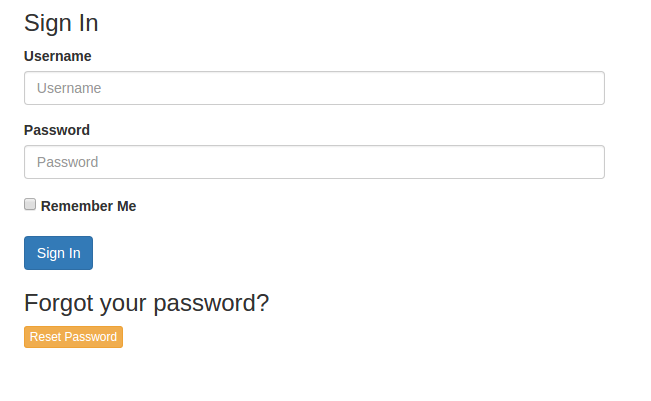
\includegraphics[width=\textwidth,height=\textheight,keepaspectratio]{diagrams/login_page}
\caption{The login page. Reset password is at the bottom.}
\label{fig:login_page}
\end{figure}

\subsection{The Main Navigation Bar}

Most navigation will be done through the use of the main navigation bar at the top of the screen, see 
Figure \ref{fig:nav_bar}. The navigation bar's content will change based on the permissions of your
account. Figure \ref{fig:nav_bar} shows an account that occupies all three roles, student, grader, and
instructor.

\begin{figure}[h]
\centering

\includegraphics[width=\textwidth,height=\textheight,keepaspectratio]{diagrams/main_header}
\caption{The main navigation bar}
\label{fig:nav_bar}
\end{figure}

From right to left the links on the navigation bar are:
\begin{description}
\item[Home] Takes you to the main page.
\item[Courses] Presents a drop-down menu which can take you to the homepage for active courses in the system.
\item[Active Grutors] Takes you to a page which shows where the current active grutors are for 
courses you are involved with (enrolled, grading, or teaching).
\item[Student] This only appears if you are a student in a course and will present a drop-down that can take
you to the problem submission page for your course or a summary of your grades.
\item[Grader] This only appears for graders and instructors of a course. It presents a drop-down for choosing
which course you want to grade assignments for.
\item[Instructor] This only appears for instructors. It presents a drop-down for which course you want to 
edit settings for.
\item[Leave a Comment] Takes you to a feedback page. Feedback provided through this page is sent to the
admin.
\item[Report a Bug] Takes you to the github issues page for the \csgt system.
\item[\textless username\textgreater] Presents a drop-down for account settings and logging out.
\end{description}


\section{Student Use}
The primary actions students will take in \csgt is submitting homework assignments and checking grades.

\subsection{Submitting Homework}
To submit homework start by clicking the \emph{Student} link on the navigation bar and selecting the course
which you want to submit work to. This will bring you to a page like in figure \ref{fig:problem_list}.

\begin{figure}[h]
\centering
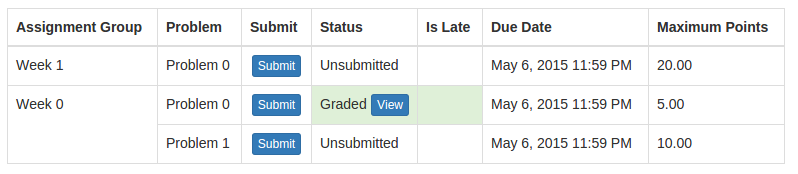
\includegraphics[width=\textwidth,height=\textheight,keepaspectratio]{diagrams/problem_list}
\caption{A list of problems for a course. Problems are grouped by \textbf{Assignment Group}}
\label{fig:problem_list}
\end{figure}

Problems are grouped by \textbf{Assignment Group} which may refer to single weeks or any other logical
grouping of multiple problems. Assignment groups are displayed in reverse order so that the most recently
assigned group is at the top of the list and thus easier to find.

Once you have located the problem you wish to submit click the blue \emph{Submit} button. This will direct 
you to a page like in figure \ref{fig:submit_page}.

\begin{figure}
\centering
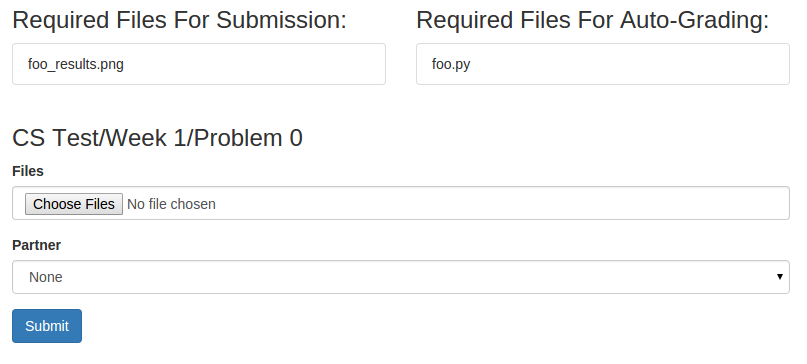
\includegraphics[width=\textwidth,height=\textheight,keepaspectratio]{diagrams/submit_page}
\caption{The page for submitting files for a problem}
\label{fig:submit_page}
\end{figure}

On the submit page there is information about what files are expected, a place for you to choose the
files you are submitting and a drop-down to select an optional partner.

\begin{description}
\item[Required Files For Submission] These files must be present in the set of files you select or else 
the system will reject the submission.
\item[Required Files For Auto-Grading] If any of these files are not present the submission will be accepted
but the auto-grader will not run. 
\item[Files] Will open a file selection window. To submit multiple files you may either select multiple files in
the window, or submit a zip file. If you need to preserve directory structure submit a zip file.
\item[Partner] A drop-down of all the students in the course for selecting a partner. If you select a partner
your partner does not have to submit the solution as well.
\end{description}

\subsection{Viewing Grades}
There are two ways to view grades. First on the problem list page, see figure \ref{fig:problem_list}, you can
click the \emph{view} button to see the grade and grader comments for an individual problem. 

If you want an overview of all of your grades you can go to the \emph{My Grades} page which is under the student
drop-down menu. The My Grades page will display something like in figure \ref{fig:my_grades}.

\begin{figure}
\centering
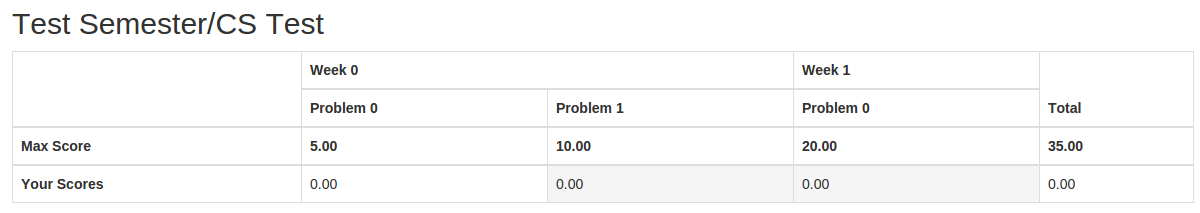
\includegraphics[width=\textwidth,height=\textheight,keepaspectratio]{diagrams/my_grades}
\caption{The My Grades page}
\label{fig:my_grades}
\end{figure}

\section{Grader Use}
\label{sec:graders}
Graders can assign grades in one of two ways, they can grade submitted assignments, or they can enter
external grades into the grade-book. This section will cover both of these options. 

\subsection{Grading Submitted Homework}
First to grade a student's submitted work click the \emph{Grader} drop-down from the navigation bar 
(see Figure \ref{fig:nav_bar}) select the course you wish to grade. This will bring up a list of all the 
problems currently assigned as seen in Figure \ref{fig:grutor_problems}.

\begin{figure}[h]
\centering
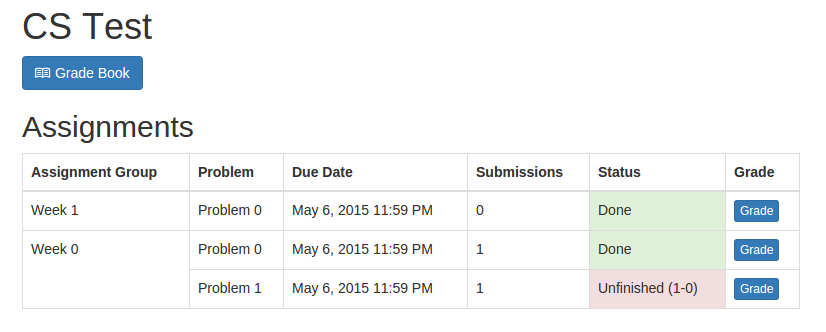
\includegraphics[width=\textwidth,height=\textheight,keepaspectratio]{diagrams/grutor_problems}
\caption{A list of all currently assigned problems in CS Test and the current grading status of the problems}
\label{fig:grutor_problems}
\end{figure}

On this page click the \emph{Grade} button for the problem you wish to grade. This will bring up a list of all
of the students in the class with the status of their submission, see Figure \ref{fig:grutor_problem_list}. 

\begin{figure}[h]
\centering
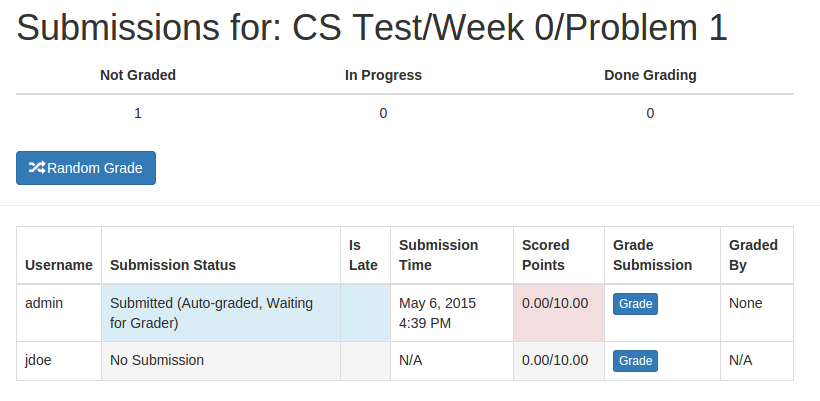
\includegraphics[width=\textwidth,height=\textheight,keepaspectratio]{diagrams/grutor_problem_list}
\caption{The current status of grading for all submissions in this problem}
\label{fig:grutor_problem_list}
\end{figure}

There are two ways to claim a submission to grade. First, you can click the \emph{Random Grade} button.
This button will atomically select a currently ungraded assignment for you. Second, you can click the 
\emph{grade} button for the student you wish to grade. Once you have selected a problem to grade you will
see a page like in Figures \ref{fig:grade_page_top} and \ref{fig:grade_page_bottom}.

\begin{figure}
\centering
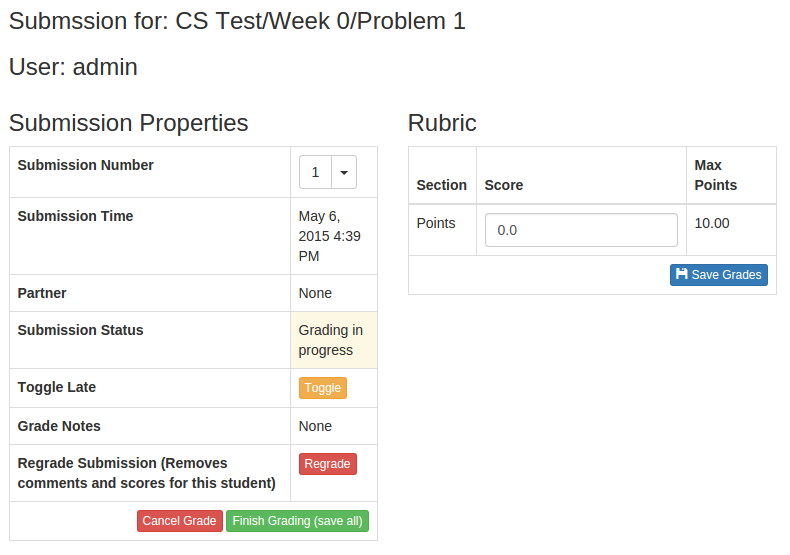
\includegraphics[width=\textwidth,height=\textheight,keepaspectratio]{diagrams/grade_top}
\caption{The top of the grading page}
\label{fig:grade_page_top}
\end{figure}

\begin{figure}
\centering
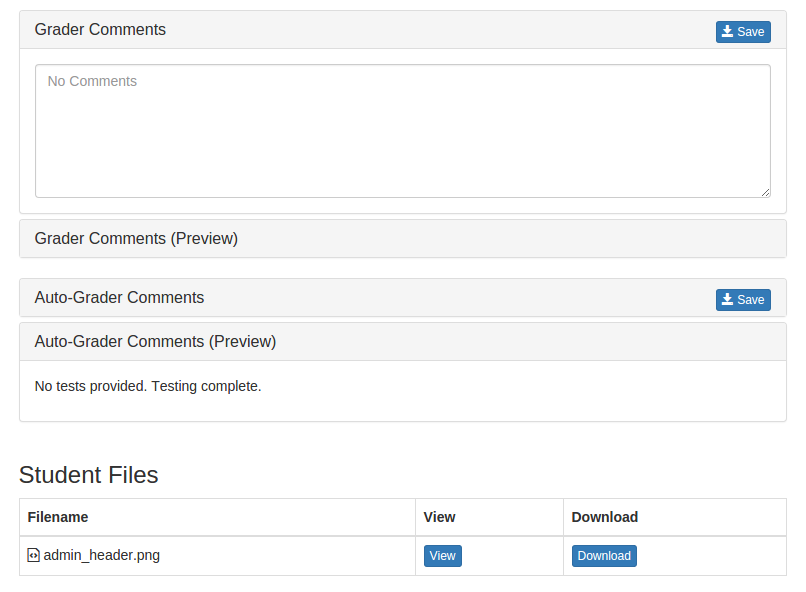
\includegraphics[width=\textwidth,height=\textheight,keepaspectratio]{diagrams/grade_bottom}
\caption{The comments and files section of the grading page}
\label{fig:grade_page_bottom}
\end{figure}

Grading is fairly simple, using the list of student files (Bottom of Figure \ref{fig:grade_page_bottom}) you
can view most textual, image, and PDF files. Files that cannot be directly viewed in browser may be
downloaded. 

To help during grading the professor can supply grading notes. These notes are in the \emph{Submission Properties}
table in the row labelled \emph{Grade Notes} (See Figure \ref{fig:grade_page_top}). If notes are supplied a button 
will be presented which will open the specified link in a new tab.

Once you have assessed the students submission and left comments (Figure \ref{fig:grade_page_bottom}) you must
save your changes and mark the submission as graded. All of this is handled by clicking the green
\emph{Finish Grading (save all)} button. Clicking this button will save all of the fields on the page and 
take you back to the list of submissions (Figure \ref{fig:grutor_problem_list}).

\noindent\textbf{Note:} If the submission you are working on has a partner that submission will receive the
exact same grades and comments that you put on this submission.

Additional things you can do on the grade page are modifying the late status of a submission, sending the
submission through the auto-grader again, and viewing old versions of the submission. These functions are 
all found in the \emph{Submission Properties} table (Figure \ref{fig:grade_page_top}).

\subsubsection{Status of Grading}

It is important to understand the different stages of grading for a submission. Each submission can be in
one of six stages:
\begin{enumerate}
\item Unsubmitted
\item Submitted: No auto-grading or grading
\item Auto-grading in progress
\item \label{item:autograded} Submitted: Auto-graded but not graded
\item \label{item:inprogress} Grading in progress
\item \label{item:graded} Graded
\end{enumerate}

Along with the status a submission also has a grader associated with it. For the most part submissions will always 
be in state \ref{item:autograded} when a grade gets to them. 
The largest area of confusion is how the \emph{Cancel Grade} and \emph{Finish Grading} buttons affect the
status of the submission. There are simple rules for how this works:
\begin{itemize}
\item You are listed as the grader of the submission.
\begin{description}
\item[Finish Grading] Sets the status to \ref{item:graded}. You are still the grader.
\item[Cancel Grading] Sets the status to \ref{item:autograded}. The submission has no grader.
\item[Leaving the page (other links)] Submission status does not change. Grader does not change.
\end{description}
\item Another grader is listed as the submission's grader
\begin{description}
\item[Finish Grading] Sets the status to \ref{item:graded}. You are now the grader.
\item[Cancel Grading] Submission status does not change. Grader does not change.
\item[Leaving the page (other links)] Submission status does not change. Grader does not change.
\end{description}
\end{itemize}

It is important to remember that if you leave the page via \emph{Cancel Grade} or any other link
none of your changes will be saved. If you want to make changes and leave with these methods you must
use the explicit blue save buttons for each section you modify.

\subsection{Entering grades in the Grade-book}
The other way graders can assign grades is through the grade-book. The grade-book is intended for assigning
grades to assignments or other parts of the class that were not submitted through the system, (e.g. 
Participation, Quizzes, Tests...).

To get to the Grade-Book click the Grader drop-down menu and select the course you wish to grade. This
brings up a page like in Figure \ref{fig:grutor_problems}. On this page click the \emph{Gradebook} button.
This will display a page like in Figure \ref{fig:gradebook}.

\begin{figure}
\centering
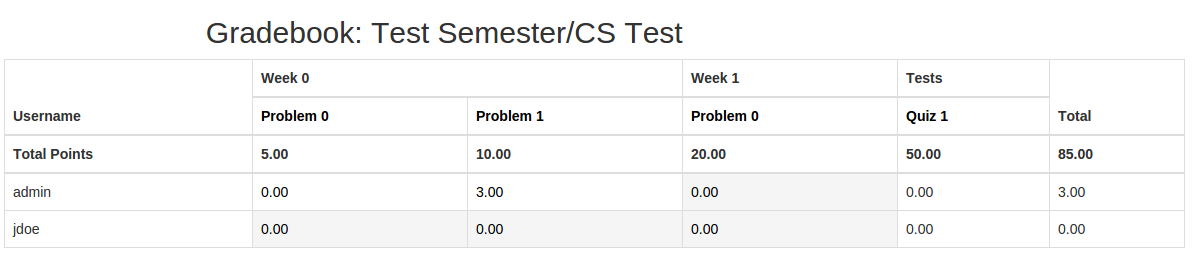
\includegraphics[width=\textwidth,height=\textheight,keepaspectratio]{diagrams/gradebook}
\caption{The grade-book for the course CS Test}
\label{fig:gradebook}
\end{figure}

Non-submitted grade-book columns are always the right most columns in the grade-book. For example in 
Figure \ref{fig:gradebook} The column \textbf{Quiz 1} in the category \textbf{Tests} is a non-submitted
column. 

To assign grades click the name of the column, in this case \textbf{Quiz 1}. This will take you to a page
like seen in Figure \ref{fig:gradecolumn}.

\begin{figure}
\centering
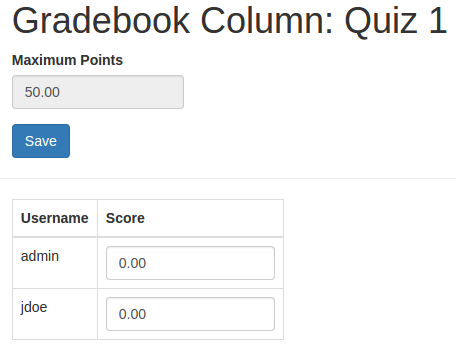
\includegraphics[width=\textwidth,height=\textheight,keepaspectratio]{diagrams/gradecolumn}
\caption{The grade column for Quiz 1 in CS Test}
\label{fig:gradecolumn}
\end{figure}

From here you may edit each students score. When you are done you can press save and leave. 
\textbf{Important Note:} Two graders cannot be editing the same grade-book column at the same time
once one grader saves their changes it will overwrite the other graders changes.

\pagebreak
\section{Instructor Use}
Instructors are responsible for configuring problems and adding columns to the grade-book as well as grading.
Since grading was covered in Section \ref{sec:graders} this section will focus on configuring courses and 
problems.

\subsection{General Course Settings}
Once an administrator has created a course and assigned you as an instructor you will need to begin configuring
your course. The course settings page is shown in Figure \ref{fig:course_settings}, this section will describe
the functionality of this page. \textbf{Note:} The figure does not show the entire page. At the bottom of the
page is the list of students, grutors, and instructors. This document will explain later how to use these lists.

First let us examine the \emph{Settings} panel near the bottom of the page. There are three major settings for
a course.

\begin{description}
\item[Course Homepage] This setting changes where the link in the \emph{Courses} drop down from the nav-bar
goes. By default it links to an empty built-in wiki page (use of the wiki is described in Section \ref{sec:wiki})
but it can be changed to link to an external site.
\item[Use Anonymous Grading] This boolean setting changes whether or not usernames are made anonymous to 
graders. If it is active any page under the \emph{Grader} drop-down for this course will use anonymous usernames. 
All pages in the \emph{Instructor} drop-down for this course will display both usernames.
\item[Late Work Policy] The late work policy changes how the system handles scoring assignments submitted late.
The default is \emph{Highlighter} which simply highlights late assignments red in the grade book. This policy can
be replaced via plug-in to modify scores based on how late or how many late assignments a student has turned in.
\end{description}

\noindent\textbf{Note (Possible feature request):} Currently the modified grade calculated by the late policy
is only displayed in the grade-book or the students \emph{My Grades} page. If a student views a problem 
individually it will show the original grade for that problem. This may be fixed in future versions of the
\csgt system.

\begin{figure}
\centering
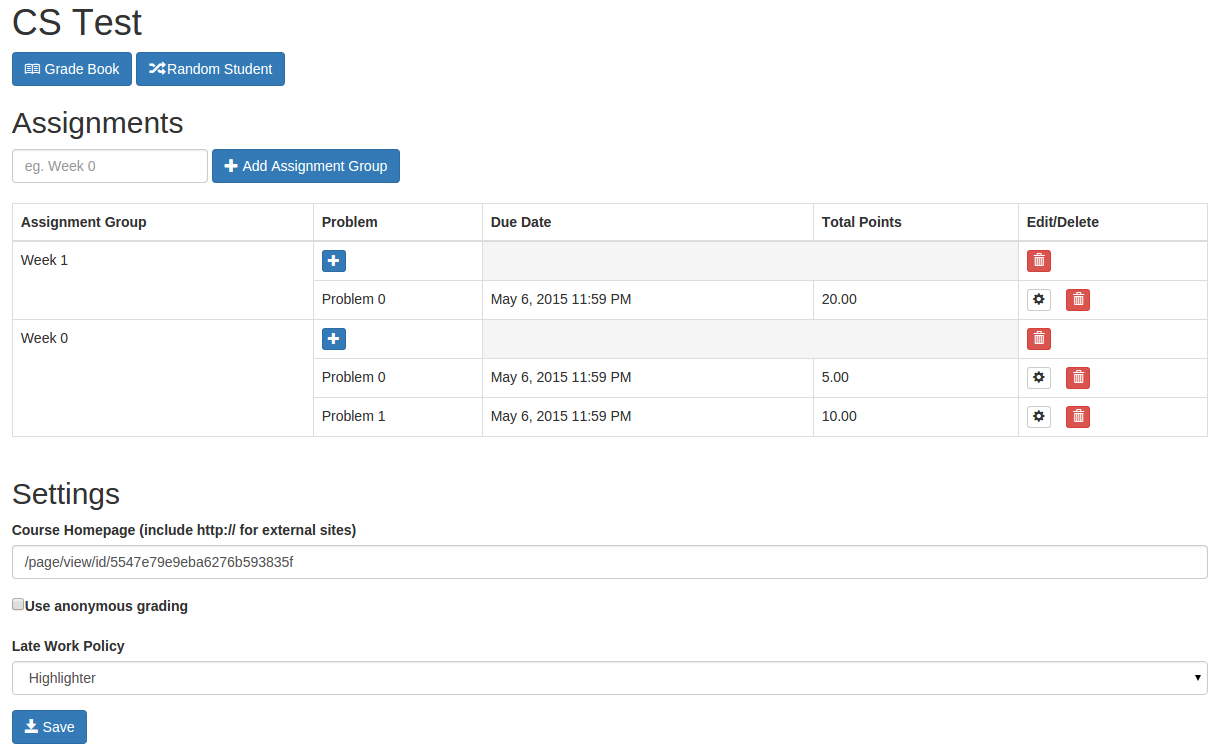
\includegraphics[width=\textwidth,height=\textheight,keepaspectratio]{diagrams/course_settings}
\caption{The main course settings page, minus the users lists}
\label{fig:course_settings}
\end{figure}

\subsection{Adding Problems}
Once you have configured the course to have the settings you want you will want to add problems.
Within the \csgt system problems are always contained within an \textbf{assignment group}. Assignment 
groups are ways to logically group related problems. For example assignment groups could be based on which week
the problems material relates to, which chapter of the book they relate to, or what problem set they are from.
Assignment groups are always displayed with the most recently assigned at the top of the page. This helps
students quickly locate the most relevant assignments.
	
To add a problem you must first create an assignment group. To create an assignment group type in the text-box
that displays the place-holder text \emph{eg. Week 0} and press the \emph{Add Assignment Group} button. In
Figure \ref{fig:course_settings} we can see that this course has assignment groups \textbf{Week 0} and 
\textbf{Week 1}. 

Once you have created an assignment group you can add a problem by clicking the blue plus button in the 
problem column for the assignment group you want. This will take you to the \textbf{Problem Settings} page, 
explained in Section \ref{sec:problem_settings}, you can also get to the problem settings page by clicking
the grey cog button for the problem you wish to modify.

\subsection{Problem Settings}




\section{Wiki Use}
\label{sec:wiki}


\chapter{Administration}
\label{ch:admin}
\section{Server Structure}
The \csgt system is designed to be modular and expandable as the number of users of the system grows. 
To accommodate this each of the five major components are designed to be operated as a separate server. 
The five components are:

\begin{enumerate}
\item Python-Flask Front-end Server
\item Python-Celery Grading Worker
\item File-system for submission storage (pick your favorite one)
\item MongoDB for storing grades
\item RabbitMQ for passing grading requests to workers
\end{enumerate}

In the most basic configuration, which is most useful for testing, all of the required components will be 
on one machine. As the requirement for redundancy and scalability increases components may be moved to 
separate servers and replicated. Figure \ref{fig:layout} shows one possible configuration of the servers
which provides redundancy on both the front and back end. It is important to note that a load-balancer is
required to support multiple front-ends.

\textbf{Note:} Currently even though MongoDB and rabbitMQ support distributed options the system has never 
been tested using that configuration. This is a feature which may be researched in the future if it becomes
needed.

\begin{figure}
\centering
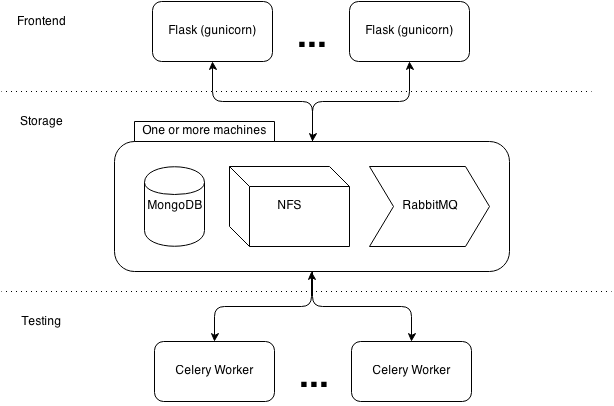
\includegraphics[width=\textwidth,height=\textheight,keepaspectratio]{diagrams/HMC_Grader_Layout}
\caption{Possible server configuration for \csgt}
\label{fig:layout}
\end{figure}





\section{Set-up}
Once you have decided on the basic configuration for your servers setting up the requisite systems requires a
little work. For each server type I will provide basic set-up instructions. These instructions are listed in 
order to prevent dependency issues. 

\subsection{MongoDB Set-up}
To set-up a brand new MongoDB instance you can use the instructions below. If you already have a running version
of MongoDB you can adapt the instructions or request help from your database administrator.
\begin{enumerate}
\item Get the latest version of MongoDB from \href{http://docs.mongodb.org/manual/tutorial/install-mongodb-on-ubuntu/}{here}.
\item Follow \href{http://docs.mongodb.org/manual/tutorial/enable-authentication/}{these} instructions to create an administrator account.
\item Edit \verb|/etc/mongodb.conf| so that 
\verb|bind_ip| is commented and uncomment
\verb|auth = true|. Additionally it is recommended to change the port that the server listens on
to prevent attacks.
\item Reload \emph{mongod} and log into the \emph{mongo} shell with\\
\verb|$ mongo -u {username} -p --authenticationDatabase admin|
\item Type \verb|> use submissionsite| to create the \emph{submissionsite} database
\item Add a user for this database by typing
\begin{verbatim}
> db.createUser(
  { user: "grader", 
    pwd: "{your password}",
    roles: [{role: "dbOwner", db: "submissionsite"}] 
  }
)
\end{verbatim}
\item Finally \verb|> quit()| the mongo shell.
\end{enumerate}

\subsection{File-system Set-up}
Setting up the file-system is pretty easy. There are two major requirements for the file-system, one, it
must be accessible from all machines in the cluster, and two it must have a minimal required directory
structure.

Because exporting a directory is complicated and other better resources exist on the internet I leave
figuring out how to export your directory as an exercise to the reader.

Once you decide how to export your chosen storage directory you must give it some basic structure. This
structure is as follows:

\begin{itemize}
	\item submissions
	\item photos
	\item plugins
	\begin{itemize}
		\item autograder
		\item latework
	\end{itemize}
\end{itemize}

Once these paths exist in your storage directory you are good to go.

\subsection{RabbitMQ Set-up}

RabbitMQ is a distributed queue which handles sending auto-grading requests to the various celery workers.
Setting up this part of the system can be very easy but depending on your security requirements you may want
to enforce more stringent permissions. To set-up RabbitMQ do the following:

\begin{enumerate}
\item Install \emph{rabbitmq-server}.
\item Run\\ \verb|$ sudo rabbitmqctl add_user {username} {password}|
\item Run\\ \verb|$ sudo rabbitmqctl set_permissions -p / {username} ".*" ".*" ".*"|
\end{enumerate}

RabbitMQ is now in a very basic workable configuration.

\subsection{Create config.py}
\label{sec:config}
The \texttt{config.py} file handles all of the connection configuration for the system.
Inside \texttt{config.py} there are several sections that need to be modified using configuration 
information from the steps above.

\begin{enumerate}
\item Give your own \verb|SECRET_KEY|
\item Configure MongoDB connection properties
\begin{verbatim}
MONGODB_SETTINGS = {
'DB': 'submissionsite',
'username': '{dbuser}',
'password': '{dbpassword}',
'host': '{db_ip}'
'port': '{db_port}'
}
\end{verbatim}
\item Configure the Celery broker URL\\
\verb|CELERY_BROKER_URL="amqp://{rabbit_user}:{rabbit_pwd}@{rabbit_ip}"|
\item Set the where the file-system will be mounted for the front/back-end servers\\
\verb|STORAGE_HOME="{path_to_mount_point}"|\\
\textbf{Note:} If you are storing the data locally you still have to set this flag but instead
want to set \verb|STORAGE_MOUNTED=False|. This disables a check to make sure that the directory is
mounted before performing writes.
\item Set up the system email (This is used for sending password reset requests
\begin{verbatim}
SYSTEM_EMAIL_ADDRESS = "{server_email}"
SMTP_SERVER = "{smtp_server}"
\end{verbatim}
\end{enumerate}

This configuration file should be passed to all front/back-end servers.
\\
\\
\noindent\textbf{Note:} There is an additional setting \verb|GRADER_USER| which is currently set to 
\verb|None|. This setting is supposed to set which user to switch to as the auto-grader but it
is currently non-functional.

\subsection{Flask Front-end Set-up}
The Flask based Front-end of the system serves dynamically generated web-pages to the users.
To set-up the flask front-end do the following:

\begin{enumerate}
\item Ensure that \verb|python-dev| (or its equivalent package) is installed on your platform.
\item Check out the repository
\item \verb|$ cd <your_repository>|
\item Copy \texttt{config.py} to the repository
\item Create a virtual environment using \verb|virtualenv <venv_name>|
\item \textbf{Temporary Fix} The current version of mongoengine does not function with the latest version
of pymongo. To solve this install version 2.8 \verb|$ <venv_name>/bin/pip install pymongo==2.8|
\item Install the following packages with pip\\
\texttt{\$ <venv\_name>/bin/pip install flask flask-script flask-bootstrap flask-login flask-markdown mongoengine flask-mongoengine WTForms python-dateutil celery psutil python-magic bleach gunicorn gevent flower}
\item Launch the front-end processes\\
\verb|$ <venv_name>/bin/celery flower -A app:celery|\\
\verb|$ <venv_name>/bin/gunicorn -w 4 -k gevent -b 0.0.0.0:80 app:app|
\end{enumerate}

\noindent\textbf{Note:} You may have to modify some permissions to allow \emph{gunicorn} to bind to port 80. 
Additionally if you are using a load balancer you may want to bind it to some other higher port.

\subsection{Celery Worker Back-end Set-up}
Setup for the Celery Worker is almost identical to the Flask front-end but requires fewer packages. The
instructions are displayed below:

\begin{enumerate}
\item Ensure that \verb|python-dev| (or its equivalent package) is installed on your platform.
\item Check out the repository
\item \verb|$ cd <your_repository>|
\item Copy \texttt{config.py} to the repository
\item Create a virtual environment using \verb|virtualenv <venv_name>|
\item \textbf{Temporary Fix} The current version of mongoengine does not function with the latest version
of pymongo. To solve this install version 2.8 \verb|$ <venv_name>/bin/pip install pymongo==2.8|
\item Install the following packages with pip\\
\texttt{\$ <venv\_name>/bin/pip install flask flask-script flask-bootstrap flask-login flask-markdown mongoengine flask-mongoengine WTForms python-dateutil celery psutil python-magic bleach}
\item Launch the worker processes\\
\verb|$ <venv_name>/bin/celery worker -A app:celery|
\end{enumerate}

\subsection{Bootstrap the Administrator Account}
All of the previous sections have gotten a working version of the system but currently there are no accounts
in the database. To begin creating accounts there must be an administrator account. 

The easiest way to create the \texttt{admin} account is to run\\
\verb|$ <venv_name>/bin/python run.py|\\
then kill this process. \texttt{run.py} launches the debug server which also checks for an administrator account
if no account is found it creates it. You can find the password for the default \texttt{admin} account in
\texttt{run.py}.





\section{Managing Courses}
\subsection{Creating Courses}
The administrator is required to create all of the courses for the system. When a course is created all administrators are invisibly added as instructors. Any other instructors must be explicitly added by an 
administrator. 

To add a new course to the system first navigate to the \emph{Admin Dashboard} (See Figure \ref{fig:admindash}).
Once in the Admin Dashboard click the link for the \emph{Courses} panel. Fill in the required information and
click the \emph{Create Course} button.

\begin{figure}
\centering
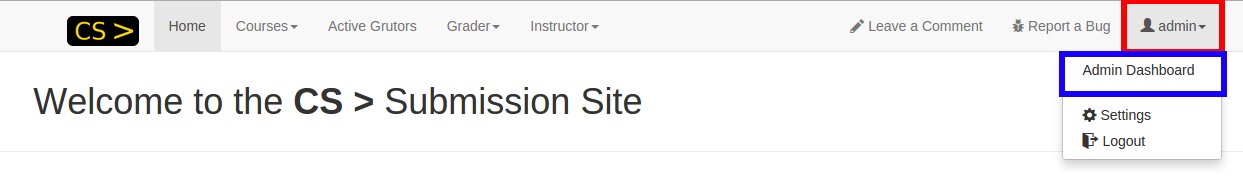
\includegraphics[width=\textwidth,height=\textheight,keepaspectratio]{diagrams/admin_header}
\caption{Red: The user Dropdown, Blue: The admin dashboard link}
\label{fig:admindash}
\end{figure}

\subsection{Adding Instructors}
Once a course has been created instructors (other than the current administrators) must be added to the course.
This requires the following actions:
\begin{enumerate}
\item Navigate to the course settings page. If you just created the course find it in the \emph{Active Courses}
list and click \emph{Administer}. If you are on the main page click the \emph{Instructor} drop-down and click on
the course link.
\item Scroll to the bottom of the course settings page. 
\item Under the instructors heading enter the user-name of the desired instructor. (If the instructor does not have an account yet see Section \ref{sec:createusers}). Click the plus button. 
\item That user is now an instructor.
\end{enumerate}

\subsection{Deactivating Courses}
When a course is finished it is desired to prevent that course from being modified. Additionally we want
currently activated courses to be prioritized when displaying lists of courses to users. 
To accomplish this \csgt allows the administrator to \textbf{Deactivate} a course. When a course is deactivated
it no longer accepts submissions and is moved from the main drop down menus into a separate page of old courses.

To deactivate a course first navigate to the Admin Dashboard and then to the Courses panel. Once on the courses
panel find the desired course and click the \emph{Deactivate} button.
\\
\\
\noindent\textbf{Note:} Some of the archival pages are still works in progress, but the framework is there to 
accomplish these features. If you run into problems with deactivated courses please submit a bug report.



\section{Creating User Accounts}
\label{sec:createusers}
One of the primary roles of the \texttt{admin} account is to create user accounts. There are two methods
for creating accounts for users. 

\subsection{Creating via web}
Web creation is the easiest way to create a small number of accounts. The steps are as follows:

\begin{enumerate}
\item Navigate to the \emph{Admin Dashboard} by clicking the user drop-down menu and then \emph{Admin Dashboard}. Figure \ref{fig:admindash} shows the locations of the links.

\item Once in the \emph{Admin Dashboard} navigate to the user panel using the top bar. (See Figure \ref{fig:adminuser})
\item Fill in the information fields and click \textbf{Create User}. (See Figure \ref{fig:adminuser})

\begin{figure}[h]
\centering
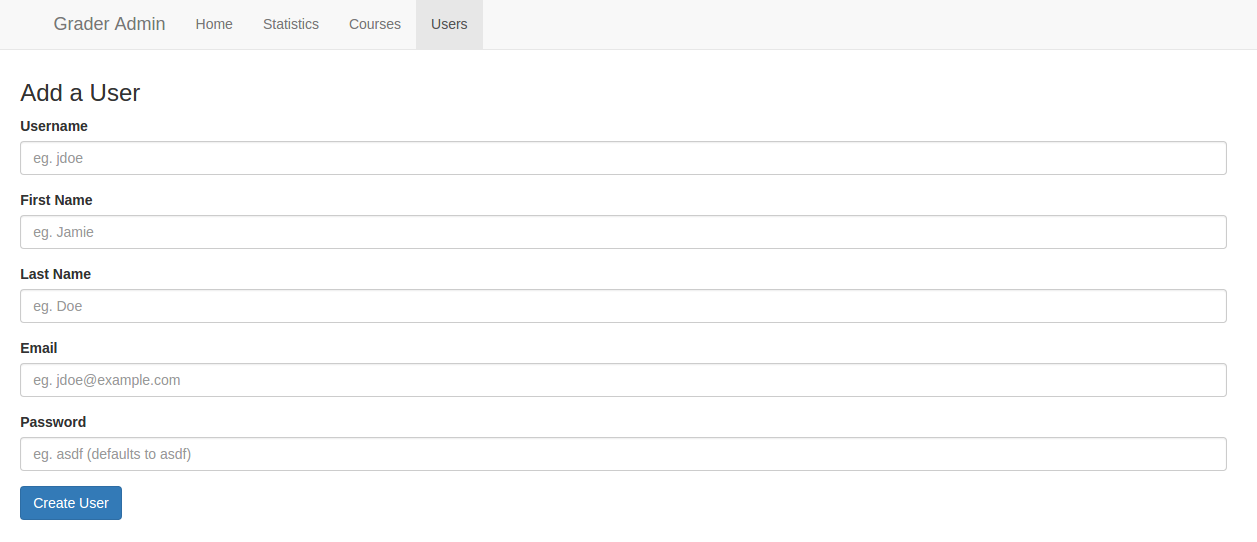
\includegraphics[width=\textwidth,height=\textheight,keepaspectratio]{diagrams/admin_users}
\caption{The admin users panel}
\label{fig:adminuser}
\end{figure}
\end{enumerate}

\subsection{Creating via command line}
Creating new users via the command line is generally one of the easiest ways to add large batches of users. 
There are already several scripts (Located in \verb|app/scripts| in the repository) which demonstrate how to 
add users from various files (CSV files with different column layouts). Below are general instructions for adding
a user via command line:
\\
\\
\noindent\textbf{Note:} To correctly use the mongo interface for the system in python you must export \verb|PYTHONPATH| as the root directory of the repository.

\begin{verbatim}
$ export PYTHONPATH=<path_to_repository>
$ <venv_name>/bin/python
...python start message...
>>> from app.structures.models.user import *
>>> user = User()
>>> user.username = "<username>"
>>> user.firstName = "<firstName>"
>>> user.lastName = "<lastName>"
>>> user.email = "<email>"
>>> user.setPassword("<password>")
>>> user.save()
\end{verbatim}

\noindent If we then want to add the user to a course we want to continue by doing

\begin{verbatim}
>>> from app.structures.models.course import *
>>> c = Course.objects.get(semester="<semester>", name="<name>")
>>> #One or more of these
>>> user.courseStudent.append(c)
>>> user.courseGrutor.append(c)
>>> user.courseInstructor.append(c)
>>> user.save()
\end{verbatim}




\chapter{Development}
\label{ch:develop}
Foo

\chapter{Command Line Reference}
Foo
\end{document}
